\iffalse
\documentclass[12pt]{article}
\usepackage{graphicx}
\usepackage{amsmath}
\usepackage{mathtools}
\usepackage{gensymb}

\newcommand{\mydet}[1]{\ensuremath{\begin{vmatrix}#1\end{vmatrix}}}
\providecommand{\brak}[1]{\ensuremath{\left(#1\right)}}
\providecommand{\norm}[1]{\left\lVert#1\right\rVert}
\newcommand{\solution}{\noindent \textbf{Solution: }}
\newcommand{\myvec}[1]{\ensuremath{\begin{pmatrix}#1\end{pmatrix}}}
\let\vec\mathbf

\begin{document}
\begin{center}
\textbf\large{CHAPTER-11 \\ CIRCLES}

\end{center}
\section{Excercise 11.1}
Find the equation of the circle with centre $(-a,-b)$ and radius $\sqrt{a^2-b^2}$.

\section{SOLUTION}
\fi
Since
\begin{align}
	\vec{c} &= \myvec{-a\\-b} \text{ and } r = \sqrt{a^2-b^2}
	\\
	\vec{u} &= \myvec{a\\b},\,
	f = \norm{\vec{u}}^2 - r^2
	  =2b^2
\end{align}
Thus, the equation of circle is 
\begin{align}
	\norm{\vec{x}}^2 +2 \myvec{a&b}\vec{x}+2b^2 &= 0       		       
\end{align}	
See Fig.
		\ref{fig:chapters/11/11/1/5/Figure} for 
\begin{align}
	a = -3, b = -2
\end{align} 
\begin{figure}[h]
\centering
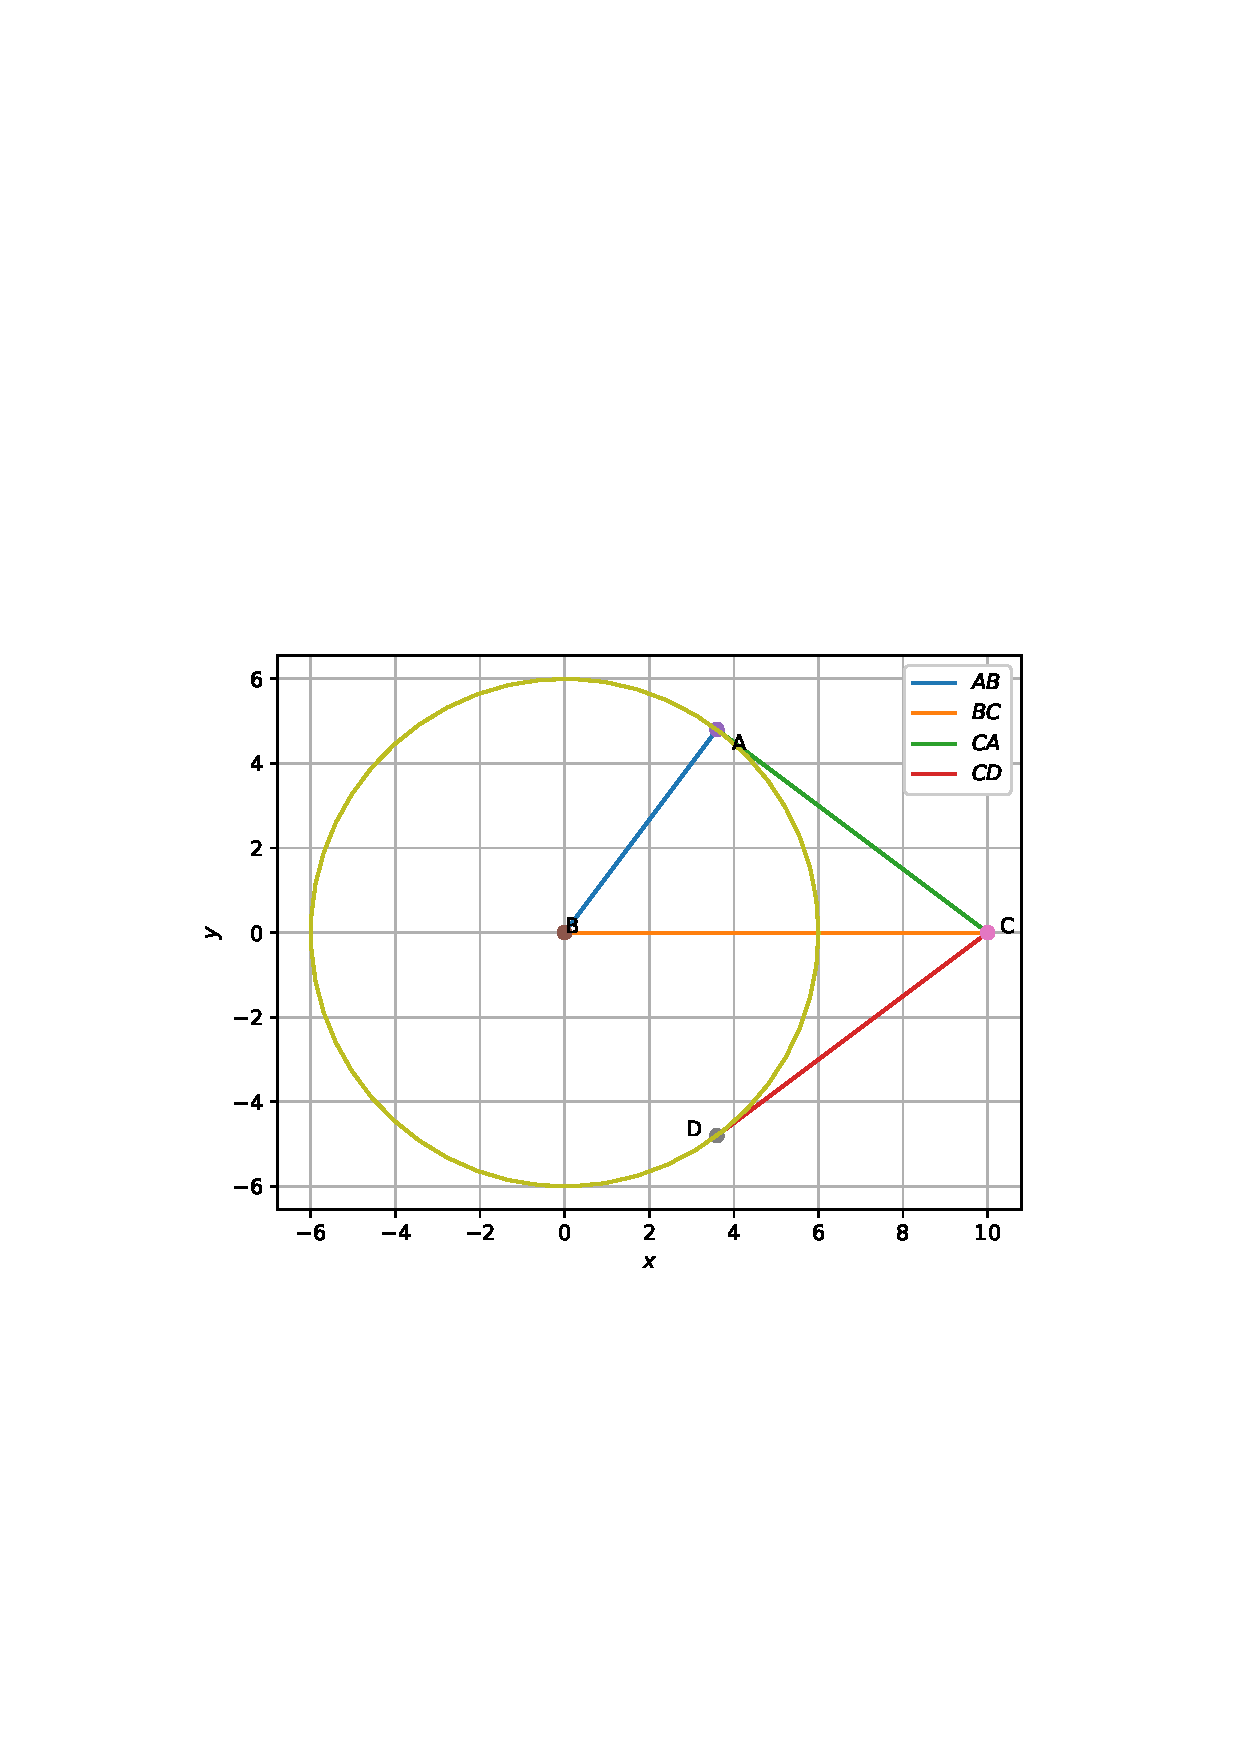
\includegraphics[width=\columnwidth]{chapters/11/11/1/5/figs/circle.png}
\caption{circle}
		\label{fig:chapters/11/11/1/5/Figure}
\end{figure}
